% 2022 A 题模拟赛论文完整稿：问题一至问题四
% 在本目录执行：latexmk -xelatex main.tex
\documentclass[withoutpreface]{../../../templates/CUMCM2026-Complete-LaTeX/cumcmthesis}

\usepackage{float}
\usepackage{mathtools}
\usepackage{siunitx}
\usepackage{tabularx}
\usepackage{booktabs}
\usepackage{enumitem}
\usepackage{tikz}
\usetikzlibrary{arrows.meta,calc,decorations.pathmorphing,positioning}

\graphicspath{{../figures/final/}}
\sisetup{detect-all}

% 按完整模版格式排版附录代码
\lstset{
  basicstyle=\ttfamily\small,
  keywordstyle=\color{blue},
  commentstyle=\color{gray},
  stringstyle=\color{teal},
  numbers=left,
  numberstyle=\tiny\color{gray},
  frame=single,
  framesep=3pt,
  breaklines=true,
  columns=fullflexible,
  keepspaces=true,
  showstringspaces=false
}

\title{波浪能装置多自由度响应与 PTO 阻尼优化}
\tihao{A}
\baominghao{}
\schoolname{}
\membera{}
\memberb{}
\memberc{}
\supervisor{}
\yearinput{2026}
\monthinput{8}
\dayinput{16}

\begin{document}

\maketitle

\begin{abstract}
针对波浪能装置中浮子--振子的多自由度响应与 PTO 阻尼优化问题，本文以静水平衡位置为基准，从动能、势能和广义耗散函数出发，建立垂荡与纵摇运动的统一动力学模型；以周期稳态平均耗散功率衡量装置的持续输出能力，并研究阻尼参数的约束最优取值。

对于问题一，选取浮子和振子的垂荡位移为广义坐标，由拉格朗日方程推导二自由度耦合模型，计算得到两种阻尼工况前 $40$ 个周期内按 $0.2\ \mathrm{s}$ 输出的完整响应。在 $100\ \mathrm{s}$ 时，按 $[x_f,v_f,x_o,v_o]$ 排列，常量阻尼工况的状态为 $[-0.0836,-0.6042,-0.0841,-0.6430]$，幂律阻尼工况为 $[-0.0884,-0.6098,-0.0935,-0.6501]$，其中位移、速度单位依次为 $\mathrm{m}$、$\mathrm{m/s}$。幂律阻尼在当前速度范围内的等效耗散较弱，因而相对运动略大；其余指定时刻及完整序列见正文结果表与支撑材料。

对于问题二，常量阻尼采用复频域稳态解，幂律阻尼采用周期射击法求取稳定周期轨道。常量阻尼的最优系数约为 $3.72\times10^4\ \mathrm{N\,s/m}$，平均功率为 $229.33\ \mathrm{W}$；幂律阻尼在 $a=1.00\times10^5$、$p=0.416$ 时取得 $229.99\ \mathrm{W}$。后者仅提高约 $0.29\%$，且比例系数达到允许上界，说明其增益受到参数边界制约。

对于问题三，在微幅波和小角度条件下，由运动学及能量关系推导四自由度线性模型，并补全物理转动惯量。在 $100\ \mathrm{s}$ 时，浮子垂荡位移、速度分别为 $-0.0502\ \mathrm{m}$、$-0.9467\ \mathrm{m/s}$，振子分别为 $-0.0426\ \mathrm{m}$、$-1.0365\ \mathrm{m/s}$；浮子纵摇角、角速度分别为 $0.0381\ \mathrm{rad}$、$0.1186\ \mathrm{rad/s}$，振子分别为 $0.0394\ \mathrm{rad}$、$0.1227\ \mathrm{rad/s}$。前 $40$ 个周期内最大垂荡位移约为 $0.916\ \mathrm{m}$，最大纵摇角约为 $0.154\ \mathrm{rad}$；直线与旋转 PTO 累计输出约为 $6.94\ \mathrm{kJ}$ 和 $1.93\ \mathrm{J}$，表明能量输出主要来自垂荡方向；其余指定时刻及完整序列见正文与支撑材料。

对于问题四，利用一阶模型的块对角结构将总平均功率严格分解为两个单变量函数，并由秩一阻尼更新推导解析最优条件。最优直线阻尼约为 $5.92\times10^4\ \mathrm{N\,s/m}$，最优旋转阻尼取上界 $1.00\times10^5\ \mathrm{N\,m\,s}$，最大总平均功率约为 $318.68\ \mathrm{W}$。频域与时域独立求解、能量平衡及全域搜索相互验证。综合结果表明，在题设参数域内幂律阻尼相对常量阻尼的功率增益有限，而装置输出由垂荡方向的直线 PTO 主导。

\keywords{波浪能\quad 拉格朗日方程\quad 周期稳态\quad 垂荡与纵摇\quad PTO 阻尼优化}
\end{abstract}

\section{问题重述}

\subsection{问题背景}

波浪能装置通过浮子与内部振子的相对运动驱动能量输出系统（power take-off，PTO）中的阻尼器做功，将波浪的机械能转化为可利用能量。在线性波浪理论下，浮子除受周期激励外，还受到附加惯性、兴波阻尼和静水恢复作用\cite{falnes2002,cummins1962}。因此，准确描述浮子、振子与 PTO 之间的耦合关系，是后续优化输出功率的基础。

\subsection{问题一的要求}

问题一只考虑浮子和振子的竖直垂荡运动。已知波浪激励力为 $f\cos(\omega t)$，角频率取 $\omega=1.4005\ \mathrm{s^{-1}}$，角度均采用弧度制。需要分别对常量阻尼系数 $10000\ \mathrm{N\,s/m}$ 和阻尼系数随相对速度绝对值的 $0.5$ 次幂变化两种工况建模，计算前 $40$ 个波浪周期内的位移和速度，并给出 $10$、$20$、$40$、$60$ 和 $100\ \mathrm{s}$ 时的指定结果。

\subsection{问题二的要求}

问题二沿用垂荡运动模型，改用 $\omega=2.2143\ \mathrm{s^{-1}}$ 的水动力参数。需分别在常量阻尼系数 $c\in[0,100000]$ 以及幂律阻尼参数 $a\in[0,100000]$、$p\in[0,1]$ 的约束下，确定使 PTO 平均输出功率最大的阻尼参数与最大功率。

\subsection{问题三的要求}

问题三允许浮子同时作垂荡和纵摇运动，振子随中轴转动并沿中轴滑动。在 $\omega=1.7152\ \mathrm{s^{-1}}$、直线阻尼系数 $10000\ \mathrm{N\,s/m}$ 和旋转阻尼系数 $1000\ \mathrm{N\,m\,s}$ 下，需建立垂荡--纵摇动力学模型，计算前 $40$ 个波浪周期内的垂荡位移与速度、纵摇角与角速度，并按 $0.2\ \mathrm{s}$ 间隔输出正式结果。

\subsection{问题四的要求}

问题四沿用垂荡--纵摇四自由度模型，采用 $\omega=1.9806\ \mathrm{s^{-1}}$ 的水动力参数。直线与旋转 PTO 阻尼系数均为常量，并分别在 $[0,100000]$ 内取值，需求使两类 PTO 总平均输出功率最大的两个阻尼系数及最大功率。

\section{问题分析}

\subsection{问题一的分析}

问题一属于外周期激励下的二自由度耗散振动问题。模型的关键有三点：一是将附加质量并入浮子的有效惯性；二是根据水线面几何确定静水恢复刚度；三是保证弹簧力与 PTO 阻尼力作为内力，在浮子和振子方程中符号相反。常量阻尼工况为线性系统，幂律阻尼工况为非线性系统，两者可在统一状态方程下进行求解和对比。

\subsection{问题二的分析}

问题二的核心是在同一周期稳态口径下极大化 PTO 平均耗散功率。常量阻尼对应线性定常系统，可利用复频域稳态解将优化化为一维问题；幂律阻尼则使系统呈现速度相关非线性，需直接求解周期轨道并在二维约束域内搜索。为避免初始自由振动影响目标值，本文不使用从零初态起算的全程平均，而使用单个稳定周期的平均功率。

\subsection{问题三的分析}

问题三将运动扩展为浮子和振子的垂荡与纵摇四自由度响应。在微幅波和小角度一阶线性化下，垂荡与纵摇之间的交叉项为二阶小量，因此整体模型可分解为垂荡和纵摇两个耦合二自由度子系统。建模难点在于由壳体几何补全物理转动惯量，并保留振子绕移动铰轴运动所导致的纵摇非对角惯性耦合。

\subsection{问题四的分析}

问题四中两类 PTO 阻尼均为常量，因此可直接在频域求周期稳态响应。由于一阶模型的垂荡与纵摇子系统块对角分离，总功率是两个各依赖一个阻尼系数的功率函数之和，二维联合优化可严格分解为两个一维有界优化。在此基础上，可由秩一阻尼更新推导解析最优点，再以全域扫描、二维随机优化和时域积分交叉验证。

\section{模型假设}

\begin{enumerate}[leftmargin=3.2em]
  \item 问题一和问题二仅考虑浮子与振子的竖直垂荡；问题三和问题四进一步考虑侧视平面内的纵摇。
  \item 海水无黏、无旋，附加质量和兴波阻尼采用题目给定的线性系数。
  \item 位移相对静水平衡位置定义，因此重力、静浮力和弹簧的静态预压缩量在增量方程中相互抵消。
  \item 浮子运动过程中水线始终位于圆柱壳体段，水线面积可取 $A_w=\pi R^2$。
  \item 忽略中轴、底座、隔层和 PTO 自身的质量，忽略题目未给出的其他摩擦。
  \item 问题三和问题四满足微幅波和小角度条件，只保留位移、转角及其导数的一阶项。
  \item 主模型将浮子视为密度均匀的封闭薄壳，计入圆柱侧面、圆锥侧面和顶部圆盖。
\end{enumerate}

\section{符号说明}

\begin{table}[H]
  \centering
  \caption{主要符号}
  \label{tab:symbols}
  \begin{tabularx}{0.92\textwidth}{cXc}
    \toprule
    符号 & 含义 & 单位 \\
    \midrule
    $x_f,x_o$ & 浮子、振子相对静水平衡位置的垂荡位移 & $\mathrm{m}$ \\
    $v_f,v_o$ & 浮子、振子的垂荡速度 & $\mathrm{m/s}$ \\
    $r,v_r$ & 振子相对浮子的位移和速度 & $\mathrm{m},\ \mathrm{m/s}$ \\
    $m_f,m_o,m_a$ & 浮子质量、振子质量和附加质量 & $\mathrm{kg}$ \\
    $b,k,k_h$ & 兴波阻尼系数、弹簧刚度和静水恢复刚度 & $\mathrm{N\,s/m},\ \mathrm{N/m}$ \\
    $D(v_r)$ & PTO 阻尼力函数 & $\mathrm{N}$ \\
    $f,\omega$ & 波浪激励力幅值和角频率 & $\mathrm{N},\ \mathrm{s^{-1}}$ \\
    $c$ & 常量阻尼系数 & $\mathrm{N\,s/m}$ \\
    $a$ & 幂律阻尼的比例系数 & $\mathrm{N}(\mathrm{s/m})^{p+1}$ \\
    $p$ & 幂律阻尼的幂指数 & 无量纲 \\
    $\overline P$ & 周期稳态平均 PTO 输出功率 & $\mathrm{W}$ \\
    $\theta_f,\theta_o$ & 浮子和振子的绝对纵摇角 & $\mathrm{rad}$ \\
    $J_{f,C},J_{o,C}$ & 浮子、振子绕自身质心横轴的转动惯量 & $\mathrm{kg\,m^2}$ \\
    $J_{o,P}$ & 振子绕下部铰轴的等效转动惯量 & $\mathrm{kg\,m^2}$ \\
    $c_z,c_\theta$ & 直线与旋转 PTO 阻尼系数 & $\mathrm{N\,s/m},\ \mathrm{N\,m\,s}$ \\
    \bottomrule
  \end{tabularx}
\end{table}

\section{问题一模型的建立与求解}

\subsection{坐标选取与参数确定}

以浮子和振子的静水平衡位置为坐标原点，规定竖直向上为正方向。记
\begin{equation}
 r=x_o-x_f,\qquad v_r=v_o-v_f .
  \label{eq:relative}
\end{equation}
坐标正方向、PTO 连接关系及纵摇角约定如图 \ref{fig:mechanical-schematic} 所示。图中弹簧与阻尼器均连接浮子和内部振子，其作用力在两物体方程中大小相等、方向相反。

\begin{figure}[H]
  \centering
  \begin{tikzpicture}[
    x=0.95cm,y=0.95cm,>=Latex,
    force/.style={-{Latex[length=2.6mm]},very thick},
    labelnode/.style={font=\small},
    body/.style={draw=black,thick,fill=blue!8},
    mass/.style={draw=black,thick,fill=orange!22}
  ]
    % 水面、浮子外形与中轴
    \draw[blue!65,thick] (-4.2,1.25)--(4.2,1.25);
    \node[blue!65,labelnode,anchor=west] at (4.25,1.25) {静水面};
    \draw[body] (-1.75,0.15) rectangle (1.75,2.55);
    \draw[body] (-1.75,0.15)--(0,-1.25)--(1.75,0.15)--cycle;
    \draw[densely dashed,gray] (0,-1.25)--(0,3.15);
    \node[labelnode] at (-1.25,0.86) {浮子};
    \draw[mass] (-0.52,0.55) rectangle (0.52,1.35);
    \node[labelnode] at (0,0.95) {振子};

    % 弹簧与阻尼器
    \draw[decorate,decoration={coil,aspect=0.55,segment length=2.4mm,amplitude=1.7mm},thick]
      (-0.72,2.35)--(-0.72,1.35);
    \node[labelnode,anchor=east] at (-0.92,1.83) {$k$};
    \draw[thick] (0.72,2.35)--(0.72,2.05);
    \draw[thick] (0.47,2.05) rectangle (0.97,1.77);
    \draw[thick] (0.72,1.77)--(0.72,1.35);
    \node[labelnode,anchor=west] at (1.02,1.90) {$D(v_r)$};

    % 垂荡方向与外载荷
    \draw[force,blue!70!black] (2.55,0.35)--(2.55,2.55)
      node[above,labelnode] {$x_f$ 正向};
    \draw[force,orange!80!black] (0.22,1.45)--(0.22,2.15)
      node[right,labelnode] {$x_o$};
    \draw[force,red!75!black] (-2.65,0.20)--(-2.65,2.05)
      node[above,labelnode] {$f\cos\omega t$};
    \draw[force,gray!80] (-3.35,2.25)--(-3.35,0.55)
      node[below,labelnode,align=center] {$b\dot x_f$\\$k_hx_f$};

    % 纵摇角与力矩约定
    \draw[force,green!55!black] (0.95,-0.78) arc[start angle=-35,end angle=45,radius=1.18];
    \node[green!45!black,labelnode,anchor=west] at (1.45,-1.55) {$\theta_f$：逆时针为正};
    \draw[force,purple!70!black] (-0.95,-0.80) arc[start angle=215,end angle=135,radius=1.18];
    \node[purple!70!black,labelnode,anchor=east] at (-1.45,-1.55) {$L\cos\omega t$};
    \fill (0,-0.05) circle (1.7pt);
    \node[labelnode,anchor=west] at (0.08,-0.05) {$O$};
  \end{tikzpicture}
  \caption{浮子--振子系统的坐标、PTO 连接与受力示意}
  \label{fig:mechanical-schematic}
\end{figure}
附件给出 $m_f=4866\ \mathrm{kg}$、$m_o=2433\ \mathrm{kg}$ 和 $m_a=1335.535\ \mathrm{kg}$，故浮子的垂荡有效质量为
\begin{equation}
  M_f=m_f+m_a=6201.535\ \mathrm{kg}.
  \label{eq:effective-mass}
\end{equation}
根据浮子与振子的总质量反算排水体积，所得静态吃水约为 $2.000\ \mathrm{m}$，水线位于圆柱段的 $0$--$3\ \mathrm{m}$ 范围内。因此水线面积为 $\pi R^2$，静水恢复刚度为
\begin{equation}
  k_h=\rho g\pi R^2\approx3.156\times10^4\ \mathrm{N/m}.
  \label{eq:hydrostatic-stiffness}
\end{equation}
题目给定 $b=656.3616\ \mathrm{N\,s/m}$、$f=6250\ \mathrm{N}$、$k=80000\ \mathrm{N/m}$，由 $\omega=1.4005\ \mathrm{s^{-1}}$ 得波浪周期
\begin{equation}
  T=\frac{2\pi}{\omega}\approx4.486\ \mathrm{s}.
\end{equation}

\subsection{基于能量与耗散的理论推导}

取广义坐标 $\boldsymbol q=[x_f,x_o]^{\mathsf T}$。由于坐标原点选在静水平衡位置，重力、静浮力及弹簧预压缩产生的常量项相互抵消，只保留增量势能。系统的动能和势能分别为
\begin{equation}
  \mathcal T=\frac12M_f\dot x_f^2+\frac12m_o\dot x_o^2,
  \qquad
  \mathcal V=\frac12k_hx_f^2+\frac12k(x_o-x_f)^2.
  \label{eq:q1-energy}
\end{equation}
为使常量阻尼和幂律阻尼共用同一推导，引入广义耗散函数
\begin{equation}
  \mathcal R=\frac12b\dot x_f^2+\Psi(v_r),
  \qquad
  \Psi(v_r)=\int_0^{v_r}D(s)\,\mathrm ds.
  \label{eq:q1-dissipation}
\end{equation}
当 $D(v_r)=a|v_r|^pv_r$ 时，$\Psi(v_r)=a|v_r|^{p+2}/(p+2)$；常量阻尼对应 $p=0$。波浪只对浮子直接做功，故广义力为 $\boldsymbol Q=[f\cos(\omega t),0]^{\mathsf T}$。代入含耗散项的拉格朗日方程
\begin{equation}
  \frac{\mathrm d}{\mathrm dt}\frac{\partial\mathcal T}{\partial\dot q_i}
  -\frac{\partial\mathcal T}{\partial q_i}
  +\frac{\partial\mathcal V}{\partial q_i}
  +\frac{\partial\mathcal R}{\partial\dot q_i}=Q_i
  \label{eq:q1-lagrange}
\end{equation}
即可得到浮子--振子的耦合运动方程。波浪激励力只直接作用于浮子，而弹簧力和 PTO 阻尼力作为内力在两式中大小相等、方向相反：
\begin{align}
  M_f\ddot x_f={}&f\cos(\omega t)-b\dot x_f-k_hx_f
  +k(x_o-x_f)+D(\dot x_o-\dot x_f),
  \label{eq:float-motion}\\
  m_o\ddot x_o={}&-k(x_o-x_f)-D(\dot x_o-\dot x_f).
  \label{eq:oscillator-motion}
\end{align}
这一推导同时给出系统机械能 $E=\mathcal T+\mathcal V$ 的变化率
\begin{equation}
  \frac{\mathrm dE}{\mathrm dt}
  =f\cos(\omega t)\dot x_f-b\dot x_f^2-D(v_r)v_r.
  \label{eq:q1-energy-balance}
\end{equation}
等式右端依次为波浪输入功率、兴波耗散和 PTO 输出功率的负值，因而后文的功率目标与动力学方程具有同一物理来源。

初始时刻两者均静止于静水平衡位置，因而
\begin{equation}
  x_f(0)=x_o(0)=\dot x_f(0)=\dot x_o(0)=0.
  \label{eq:initial-condition}
\end{equation}

\subsection{阻尼规律与物理约束}

两种工况的 PTO 阻尼力分别写为
\begin{align}
  D_1(v_r)&=10000v_r,\label{eq:linear-damping}\\
  D_2(v_r)&=10000|v_r|^{0.5}v_r.\label{eq:power-damping}
\end{align}
两种情况均满足 $D(v_r)v_r\geq 0$，即阻尼器的瞬时耗散功率非负，不会向机械系统注入能量。

\subsection{一阶状态方程与数值方法}

取状态向量 $\boldsymbol y=[x_f,v_f,x_o,v_o]^{\mathsf T}$，将式 \eqref{eq:float-motion}--\eqref{eq:oscillator-motion} 改写为
\begin{equation}
\begin{cases}
  \dot x_f=v_f,\\
  \displaystyle \dot v_f=\frac{f\cos(\omega t)-bv_f-k_hx_f+kr+D(v_r)}{M_f},\\[0.6em]
  \dot x_o=v_o,\\
  \displaystyle \dot v_o=\frac{-kr-D(v_r)}{m_o}.
\end{cases}
\label{eq:state-space}
\end{equation}
本文采用 DOP853 高阶自适应 Runge--Kutta 方法\cite{hairer1993}积分式 \eqref{eq:state-space}，相对容差取 $10^{-10}$，绝对容差取 $10^{-12}$，最大内部步长取 $0.02\ \mathrm{s}$。计算覆盖前 $40$ 个波浪周期，并按 $0.2\ \mathrm{s}$ 间隔输出，共得 $898$ 个时刻。题目指定的五个时刻均位于输出网格上，可直接取值，无需额外插值。

\subsection{求解结果与响应特征}

两种阻尼规律下的位移响应如图 \ref{fig:displacement} 所示。在初始阶段，系统的自由振动与波浪强迫振动叠加，形成明显的振幅包络；随着兴波阻尼和 PTO 阻尼不断耗散机械能，自由振动分量逐渐衰减，系统趋于以入射波浪频率为主的周期响应。

\begin{figure}[H]
  \centering
  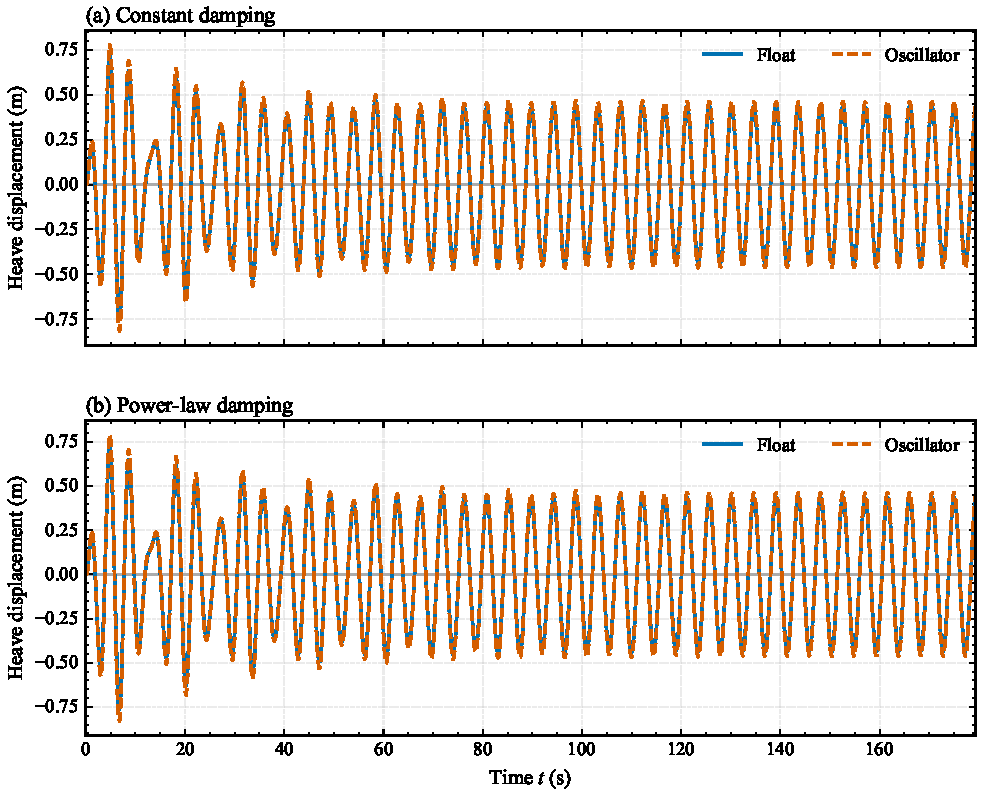
\includegraphics[width=0.96\textwidth]{q1_displacement_response.pdf}
  \caption{两种阻尼规律下浮子与振子的垂荡位移响应}
  \label{fig:displacement}
\end{figure}

速度响应见图 \ref{fig:velocity}。振子与浮子的运动趋势总体一致，但始终存在小幅的振幅差与相位差，由此产生 PTO 阻尼器做功所需的相对速度。

\begin{figure}[H]
  \centering
  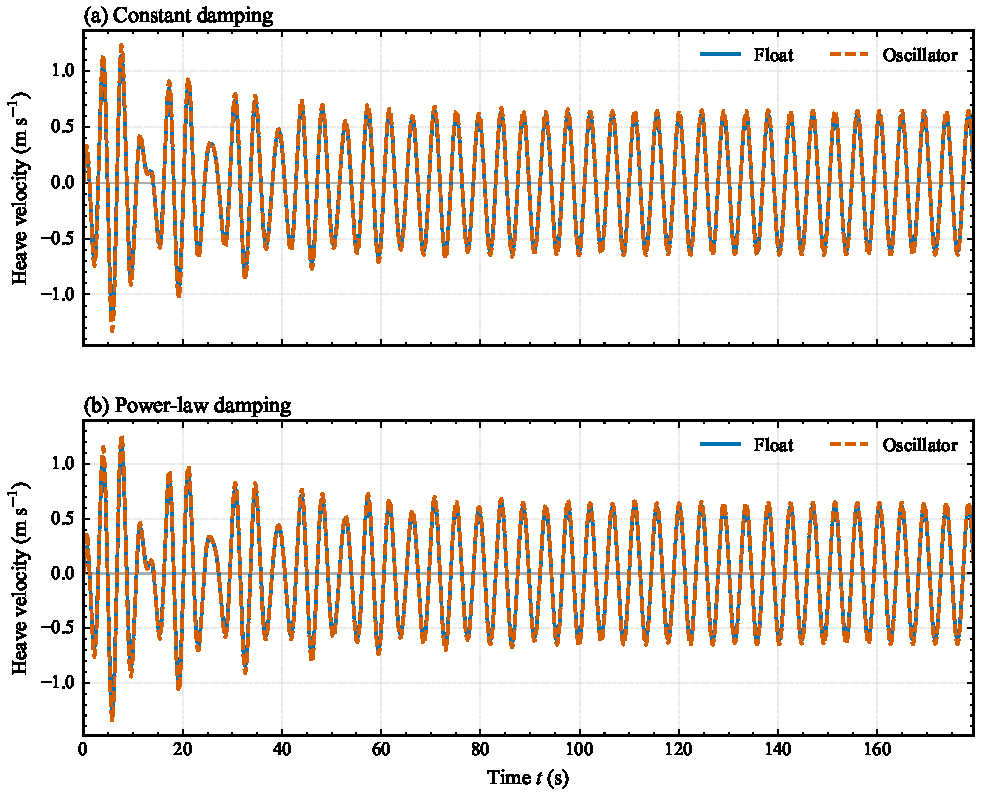
\includegraphics[width=0.96\textwidth]{q1_velocity_response.pdf}
  \caption{两种阻尼规律下浮子与振子的垂荡速度响应}
  \label{fig:velocity}
\end{figure}

常量阻尼工况在题目指定时刻的计算结果如表 \ref{tab:linear-results} 所示，幂律阻尼的相应结果如表 \ref{tab:power-results} 所示。

\begin{table}[H]
  \centering
  \small
  \caption{常量阻尼工况的指定时刻响应}
  \label{tab:linear-results}
  \begin{tabular}{ccccc}
    \toprule
    时间/s & 浮子位移/m & 浮子速度/(m/s) & 振子位移/m & 振子速度/(m/s) \\
    \midrule
    10  & -0.1907 & -0.6410 & -0.2117 & -0.6940 \\
    20  & -0.5907 & -0.2410 & -0.6342 & -0.2728 \\
    40  &  0.2854 &  0.3130 &  0.2965 &  0.3329 \\
    60  & -0.3145 & -0.4795 & -0.3314 & -0.5157 \\
    100 & -0.0836 & -0.6042 & -0.0841 & -0.6430 \\
    \bottomrule
  \end{tabular}
\end{table}

\begin{table}[H]
  \centering
  \small
  \caption{幂律阻尼工况的指定时刻响应}
  \label{tab:power-results}
  \begin{tabular}{ccccc}
    \toprule
    时间/s & 浮子位移/m & 浮子速度/(m/s) & 振子位移/m & 振子速度/(m/s) \\
    \midrule
    10  & -0.2059 & -0.6528 & -0.2346 & -0.6999 \\
    20  & -0.6111 & -0.2548 & -0.6611 & -0.2770 \\
    40  &  0.2688 &  0.2953 &  0.2802 &  0.3125 \\
    60  & -0.3272 & -0.4915 & -0.3496 & -0.5256 \\
    100 & -0.0884 & -0.6098 & -0.0935 & -0.6501 \\
    \bottomrule
  \end{tabular}
\end{table}

图 \ref{fig:relative} 展示了第 $38$--$40$ 周期的相对运动。在当前相对速度范围内，幂律阻尼的等效阻尼系数小于常量阻尼系数，因而其耗散作用相对较弱，相对位移和相对速度均略大。第 $40$ 周期内，两种工况下浮子位移半峰峰值均约为 $0.436\ \mathrm{m}$，振子位移半峰峰值约为 $0.463\ \mathrm{m}$。

\begin{figure}[H]
  \centering
  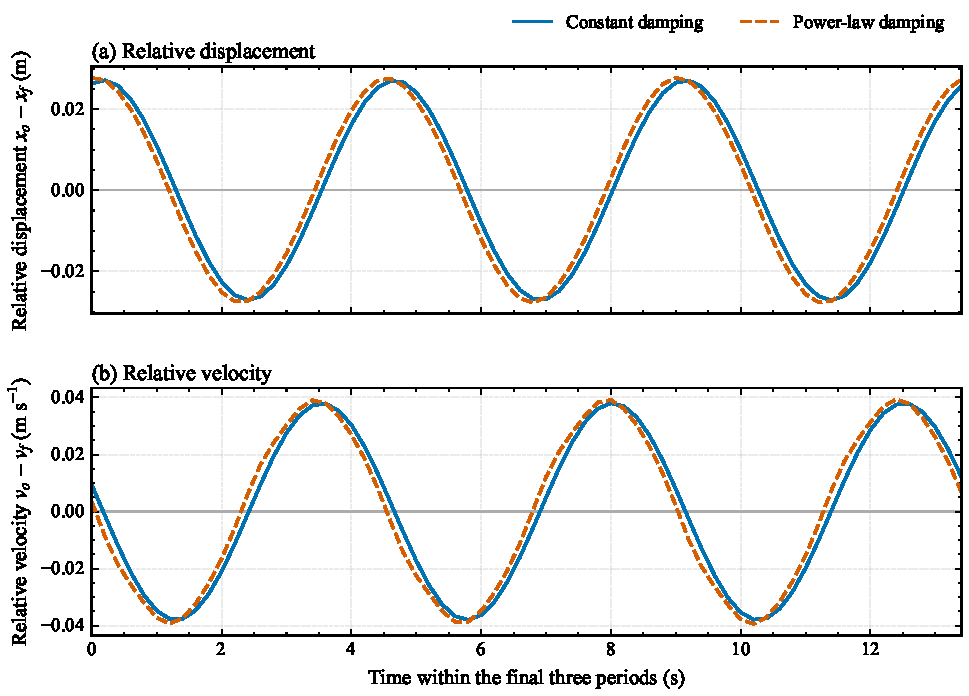
\includegraphics[width=0.96\textwidth]{q1_relative_response.pdf}
  \caption{第 $38$--$40$ 周期内两种阻尼规律的相对运动对比}
  \label{fig:relative}
\end{figure}

\subsection{模型检验}

为检验数值结果的可靠性，本文从数值收敛、能量闭合和物理适用范围三个方面进行验证。

\begin{enumerate}[leftmargin=3.2em]
  \item \textbf{数值收敛性：}将最大内部步长减半并进一步收紧积分容差，两种工况四个状态量的最大差均低于 $10^{-7}$。
  \item \textbf{能量闭合：}按式 \eqref{eq:q1-energy-balance} 计算波浪输入、机械能变化、兴波耗散和 PTO 耗散，两种工况的相对残差均低于 $10^{-12}$，说明方程符号和数值积分保持了能量一致性。
  \item \textbf{物理范围：}计算过程中圆柱段吃水始终处于 $1.276$--$2.763\ \mathrm{m}$，未超出圆柱段；弹簧长度始终为正。因此线性静水恢复力与结构几何假设在所得响应范围内自洽。
\end{enumerate}

此外，常量阻尼时域解与复频域解析稳态解达到机器精度范围内的一致，进一步从独立求解路径验证了线性工况的正确性。

\subsection{问题一小结}

本文建立的二自由度垂荡耦合模型同时包含浮子有效惯性、兴波阻尼、静水恢复力以及浮子--振子之间的弹簧和 PTO 阻尼耦合。计算得到两种阻尼规律下前 $40$ 个波浪周期的位移和速度序列，并完成了题目指定时刻的结果输出。幂律阻尼工况在当前速度范围内的相对运动略大，这一结论为问题二中以平均输出功率为目标的阻尼参数优化提供了基础。

\section{问题二 PTO 阻尼参数优化}

\subsection{优化目标与稳态口径}

问题二采用附件 3 的情形 2，其水动力参数为
\begin{equation}
  \omega=2.2143\ \mathrm{s^{-1}},\quad
  m_a=1165.992\ \mathrm{kg},\quad
  b=167.8395\ \mathrm{N\,s/m},\quad
  f=4890\ \mathrm{N}.
  \label{eq:q2-parameters}
\end{equation}
此时浮子有效质量为 $M_f=6031.992\ \mathrm{kg}$，波浪周期约为 $2.838\ \mathrm{s}$。其余结构参数与动力学方程沿用问题一。

由于本问评价装置在周期波浪下的持续输出能力，本文将目标定义为系统进入周期稳态后一个完整波浪周期内的平均 PTO 输出功率。若 $\boldsymbol y_s(t+T)=\boldsymbol y_s(t)$，则
\begin{equation}
  \overline P=\frac{1}{T}\int_{t_s}^{t_s+T}P_{\mathrm{PTO}}(t)\,\mathrm{d}t.
  \label{eq:mean-power}
\end{equation}
该口径排除了初始自由振动对优化结果的影响，使不同阻尼参数的目标值可直接比较。

\subsection{常量阻尼的复频域优化}

当 PTO 阻尼系数为常量 $c$ 时，系统为线性定常系统。定义
\begin{equation}
  \boldsymbol M=
  \begin{bmatrix}6031.992&0\\0&2433\end{bmatrix},\quad
  \boldsymbol C(c)=
  \begin{bmatrix}167.8395+c&-c\\-c&c\end{bmatrix},
  \label{eq:q2-mc}
\end{equation}
\begin{equation}
  \boldsymbol K=
  \begin{bmatrix}31557.298205+80000&-80000\\-80000&80000\end{bmatrix}.
  \label{eq:q2-k}
\end{equation}
设周期稳态位移为 $\boldsymbol x(t)=\Re\{\boldsymbol X\mathrm{e}^{\mathrm{i}\omega t}\}$，则复振幅满足
\begin{equation}
  \left(\boldsymbol K-\omega^2\boldsymbol M
  +\mathrm{i}\omega\boldsymbol C(c)\right)\boldsymbol X
  =\begin{bmatrix}4890\\0\end{bmatrix}.
  \label{eq:q2-frequency-domain}
\end{equation}
因此常量阻尼的目标函数为
\begin{equation}
  \overline P(c)=\frac{1}{2}c\omega^2
  \left|[-1,1]\boldsymbol X(c)\right|^2,
  \qquad 0\leq c\leq100000.
  \label{eq:q2-constant-objective}
\end{equation}
首先对完整可行区间进行 $10001$ 点扫描，确认目标函数只有一个内部峰值；再采用有界一维优化精修。全区间扫描、数值优化与秩一阻尼更新导出的解析最优条件相互一致，最终得到
\begin{equation}
  \boxed{c^*=3.7194\times10^4\ \mathrm{N\,s/m}},\qquad
  \boxed{\overline P_{\max}=229.334\ \mathrm{W}}.
  \label{eq:q2-constant-result}
\end{equation}

\subsection{幂律阻尼的周期射击优化}

对幂律阻尼，记比例系数为 $a$、幂指数为 $p$，则阻尼力与瞬时功率为
\begin{equation}
  D(v_r)=a|v_r|^pv_r,\qquad
  P_{\mathrm{PTO}}=a|v_r|^{p+2}\geq0,
  \label{eq:q2-power-law}
\end{equation}
其中 $0\leq a\leq100000$、$0\leq p\leq1$。由量纲一致性可知 $[a]=\mathrm{N}(\mathrm{s/m})^{p+1}$，其量纲随 $p$ 变化。为避免把 $a$ 误写成常量阻尼系数的单位，参数域图统一采用归一化横坐标 $a/a_{\max}$，其中每个给定 $p$ 下均有 $a_{\max}=100000$。

为直接定位稳定周期轨道，定义状态经过一个周期后的映射 $\boldsymbol\Phi_T$，并求解射击条件
\begin{equation}
  \boldsymbol\Phi_T(\boldsymbol y_0;a,p)-\boldsymbol y_0=\boldsymbol0.
  \label{eq:q2-shooting}
\end{equation}
得到周期初态后，将式 \eqref{eq:q2-power-law} 中的瞬时功率作为附加状态积分，便可计算目标函数
\begin{equation}
  \overline P(a,p)=\frac{1}{T}\int_0^T
  a|v_r(t;a,p)|^{p+2}\,\mathrm{d}t.
  \label{eq:q2-nonlinear-objective}
\end{equation}

优化采用“全域粗网格--脊线追踪--多起点内部精修--边界精修--最终严格复核”的分层路线。$21\times11$ 粗网格表明，高功率区域形成从低指数、低系数向高指数、高系数延伸的参数补偿脊线，如图 \ref{fig:q2-surface} 所示。橙色虚线为在各固定指数下优化比例系数得到的高功率脊线，星标为最终解。

\begin{figure}[H]
  \centering
  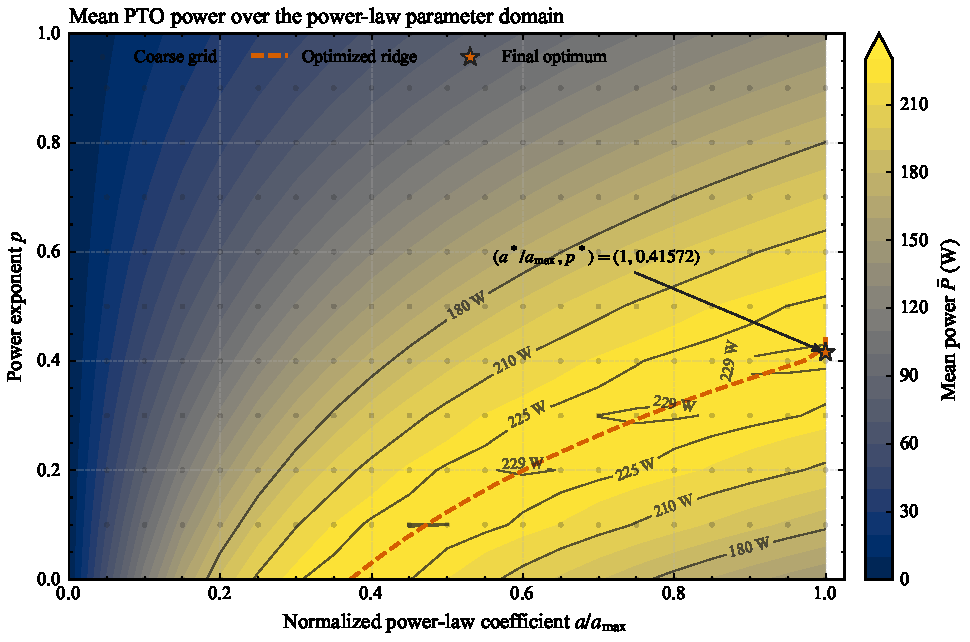
\includegraphics[width=0.94\textwidth]{q2_nonlinear_power_surface.pdf}
  \caption{归一化幂律阻尼参数域内的周期稳态平均功率与高功率脊线}
  \label{fig:q2-surface}
\end{figure}

脊线随 $p$ 增大持续向 $a$ 的上边界移动，多个内部初值也均指向同一边界。因此固定真实边界 $a=100000$，对 $p\in[0,1]$ 作 $501$ 点扫描并严格精修，最终得到
\begin{equation}
  \boxed{a^*=100000},\qquad
  \boxed{p^*=0.41572},\qquad
  \boxed{\overline P_{\max}=229.994\ \mathrm{W}}.
  \label{eq:q2-nonlinear-result}
\end{equation}
最优比例系数取到允许上界，而幂指数位于区间内部。在最优指数两侧作微小扰动，功率均下降；固定最优指数并将 $a$ 从上边界向可行域内移动，功率同样下降，说明 $a=100000$ 为活跃约束。

两类阻尼的周期稳态平均功率优化曲线如图 \ref{fig:q2-curves} 所示。常量阻尼在完整区间内只有一个内部最大值；幂律阻尼在 $a=100000$ 时，指数方向也只有一个内部峰值。

\begin{figure}[H]
  \centering
  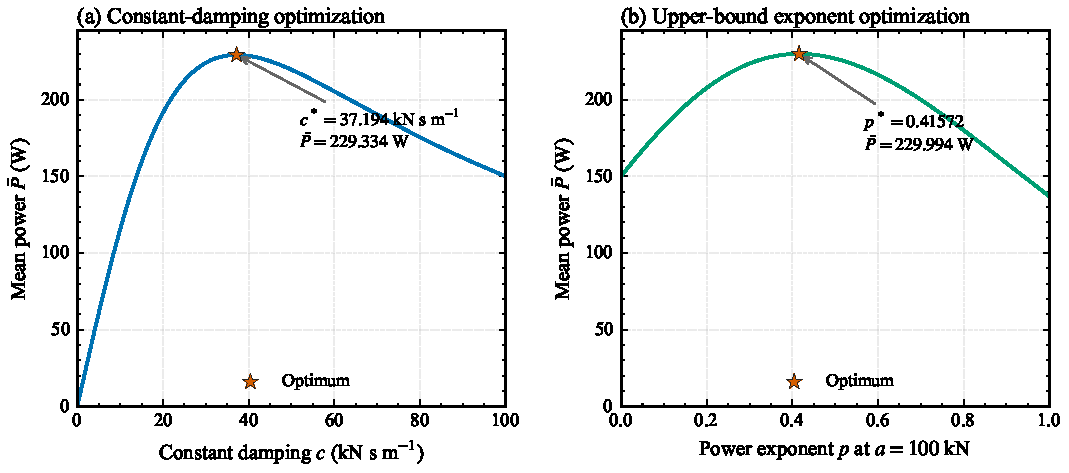
\includegraphics[width=0.94\textwidth]{q2_optimization_curves.pdf}
  \caption{两类 PTO 阻尼的周期稳态平均功率优化曲线}
  \label{fig:q2-curves}
\end{figure}

\subsection{最优结果比较}

两种阻尼规律的最优参数和最大平均功率汇总于表 \ref{tab:q2-optima}。

\begin{table}[H]
  \centering
  \caption{问题二的最优阻尼参数与最大平均功率}
  \label{tab:q2-optima}
  \begin{tabular}{ccc}
    \toprule
    阻尼形式 & 最优参数 & 最大平均功率/W \\
    \midrule
    常量阻尼 & $c^*=3.7194\times10^4\ \mathrm{N\,s/m}$ & 229.334 \\
    幂律阻尼 & $a^*=1.0000\times10^5,\ p^*=0.41572$ & 229.994 \\
    \bottomrule
  \end{tabular}
\end{table}

幂律阻尼的最大平均功率比常量阻尼提高
\begin{equation}
  229.994-229.334=0.660\ \mathrm{W},
\end{equation}
相对增幅约为 $0.288\%$。两种最优阻尼下一个稳定周期内的相对位移、相对速度和瞬时 PTO 功率如图 \ref{fig:q2-period} 所示。图中归一化时间为 $t/T$。

\begin{figure}[H]
  \centering
  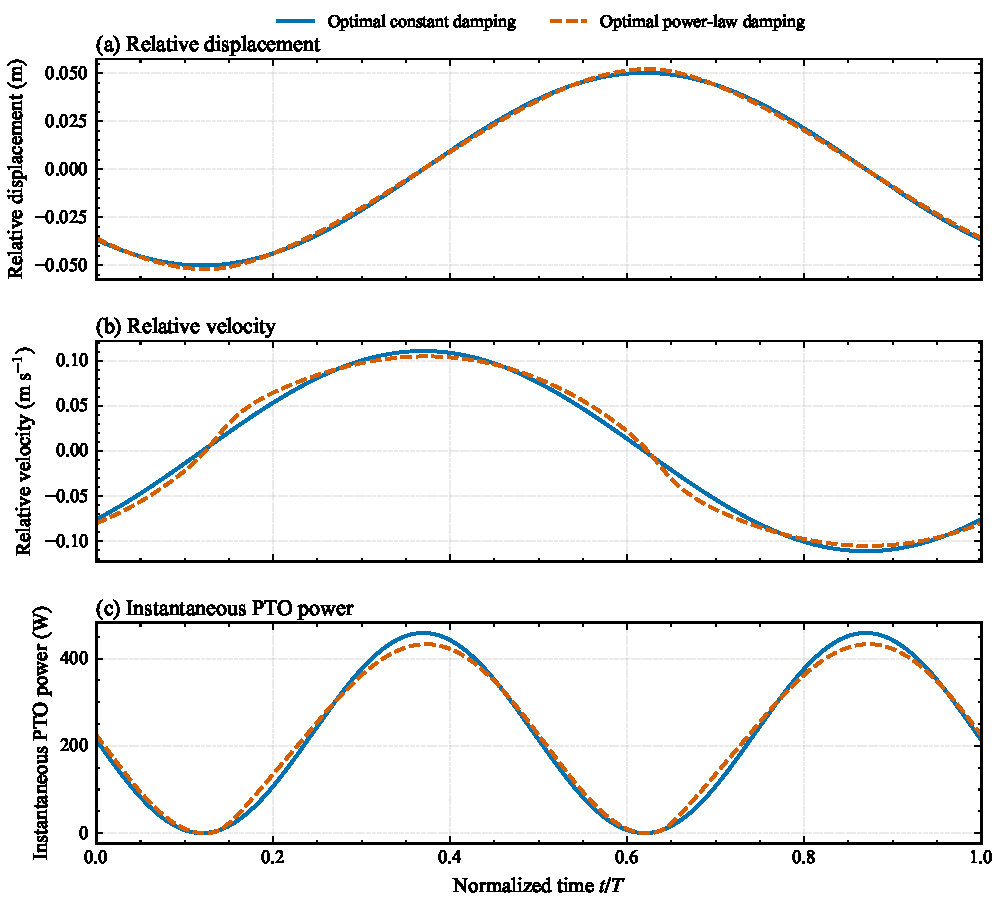
\includegraphics[width=0.94\textwidth]{q2_optimal_period_comparison.pdf}
  \caption{两种最优 PTO 阻尼下一个稳定周期的响应与输出功率}
  \label{fig:q2-period}
\end{figure}

幂律阻尼最优周期内的关键响应与物理范围汇总于表 \ref{tab:q2-period-metrics}。

\begin{table}[H]
  \centering
  \caption{幂律阻尼最优周期的关键指标}
  \label{tab:q2-period-metrics}
  \begin{tabular}{lc}
    \toprule
    指标 & 数值 \\
    \midrule
    单周期 PTO 耗散能量 & $652.62\ \mathrm{J}$ \\
    瞬时 PTO 功率最大值 & $432.91\ \mathrm{W}$ \\
    最大相对位移 & $0.0521\ \mathrm{m}$ \\
    最大相对速度 & $0.1051\ \mathrm{m/s}$ \\
    圆柱段吃水范围 & $1.551$--$2.449\ \mathrm{m}$ \\
    弹簧长度范围 & $0.150$--$0.254\ \mathrm{m}$ \\
    \bottomrule
  \end{tabular}
\end{table}

\subsection{优化结果检验}

常量阻尼最优点两侧扰动均使功率下降，复频域动力平衡残差低于 $10^{-10}\ \mathrm{N}$，时域周期解与频域功率的相对误差低于 $10^{-8}$。对幂律阻尼最优解，进一步使用三条不同的路径复核：
\begin{enumerate}[leftmargin=3.2em]
  \item \textbf{零初猜射击：}从全零周期初态启动射击，所得功率与最终严格射击结果的相对差低于 $10^{-8}$，周期轨道闭合。
  \item \textbf{冷启动长时积分：}从静水平衡零初态出发，经过充分多周期进入稳态，平均功率与严格射击结果的相对差低于 $10^{-7}$。
  \item \textbf{周期能量积分：}对最优周期内的瞬时功率直接积分，所得平均功率为 $229.994\ \mathrm{W}$，与射击结果一致。
\end{enumerate}
最优周期内 PTO 瞬时功率始终非负，吃水和弹簧长度也均满足模型的物理适用范围，说明优化结果同时满足周期稳态、能量耗散和结构几何约束。

\section{问题三垂荡--纵摇四自由度模型}

\subsection{坐标与一阶线性化}

以系统的静水平衡位置为原点，规定竖直向上为垂荡正方向，侧视平面内逆时针为纵摇正方向。记浮子和振子的垂荡位移为 $x_f,x_o$，绝对纵摇角为 $\theta_f,\theta_o$。直线 PTO 的相对位移和速度分别为 $x_o-x_f$ 和 $\dot x_o-\dot x_f$，旋转 PTO 的相对转角和角速度分别为 $\theta_o-\theta_f$ 和 $\dot\theta_o-\dot\theta_f$。

根据振子质心的平面几何关系，在微幅波和小角度条件下，垂荡与纵摇之间的交叉项为二阶小量。因此一阶模型可写为垂荡和纵摇两个块对角子系统，但纵摇子系统内部的非对角惯性项仍需保留。

\subsection{壳体几何与转动惯量}

附件仅给出浮子的纵摇附加转动惯量，物理转动惯量需结合实际转轴补全。主模型将浮子视为密度均匀的封闭薄壳，按圆柱侧面、圆锥侧面和顶部圆盖的面积分配总质量，再应用平行轴定理。得浮子质心到下部铰轴的距离和绕质心的转动惯量为
\begin{equation}
  a_f\approx1.408\ \mathrm{m},\qquad
  J_{f,C}\approx8398.78\ \mathrm{kg\,m^2}.
  \label{eq:q3-float-inertia}
\end{equation}
弹簧的静平衡长度为
\begin{equation}
  l_e=l_0-\frac{m_og}{k}\approx0.2020\ \mathrm{m},
  \label{eq:q3-equilibrium-length}
\end{equation}
故振子质心到铰轴的距离 $d=l_e+h_o/2\approx0.4520\ \mathrm{m}$。圆柱振子绕自身质心横轴的转动惯量为 $J_{o,C}=202.75\ \mathrm{kg\,m^2}$，由平行轴定理得其绕铰轴的等效转动惯量
\begin{equation}
  J_{o,P}=J_{o,C}+m_od^2\approx699.73\ \mathrm{kg\,m^2}.
  \label{eq:q3-oscillator-inertia}
\end{equation}

\subsection{纵摇运动学与能量推导}

小角度下，振子质心相对静平衡位置的水平速度为
\begin{equation}
  \dot X_O=a_f\dot\theta_f-d\dot\theta_o+O(\theta^2).
  \label{eq:q3-horizontal-velocity}
\end{equation}
其中负号来自两绝对转角的正方向与机构几何关系。于是纵摇动能为
\begin{equation}
  \mathcal T_\theta=
  \frac12(J_{f,C}+J_a)\dot\theta_f^2
  +\frac12m_o(a_f\dot\theta_f-d\dot\theta_o)^2
  +\frac12J_{o,C}\dot\theta_o^2.
  \label{eq:q3-pitch-kinetic}
\end{equation}
展开式 \eqref{eq:q3-pitch-kinetic} 可见，$-m_oa_fd\dot\theta_f\dot\theta_o$ 是移动铰轴引起的惯性耦合项；因此质量矩阵必须对称，且该非对角项不能省略。

角向势能由静水恢复、旋转弹簧和重力三部分组成。保留到转角二次项，有
\begin{equation}
  \mathcal V_\theta=
  \frac12K_h\theta_f^2
  +\frac12k_\theta(\theta_o-\theta_f)^2
  +\frac12m_oga_f\theta_f^2
  +m_ogd\cos\theta_o.
  \label{eq:q3-pitch-potential-exact}
\end{equation}
其中 $\cos\theta_o\approx1-\theta_o^2/2$，常量项不影响运动方程，故最后一项等价于 $-m_ogd\theta_o^2/2$。相应耗散函数为
\begin{equation}
  \mathcal R_\theta=
  \frac12b_\theta\dot\theta_f^2
  +\frac12c_\theta(\dot\theta_o-\dot\theta_f)^2.
  \label{eq:q3-pitch-dissipation}
\end{equation}
把式 \eqref{eq:q3-pitch-kinetic}--\eqref{eq:q3-pitch-dissipation} 代入拉格朗日方程，便得到纵摇子系统的质量、阻尼和刚度矩阵
\begin{equation}
  \boldsymbol M_\theta=
  \begin{bmatrix}
    J_{f,C}+J_a+m_oa_f^2&-m_oa_fd\\
    -m_oa_fd&J_{o,C}+m_od^2
  \end{bmatrix},
  \label{eq:q3-pitch-m-symbolic}
\end{equation}
\begin{equation}
  \boldsymbol C_\theta=
  \begin{bmatrix}b_\theta+c_\theta&-c_\theta\\-c_\theta&c_\theta\end{bmatrix},
  \quad
  \boldsymbol K_\theta=
  \begin{bmatrix}
    K_h+k_\theta+m_oga_f&-k_\theta\\
    -k_\theta&k_\theta-m_ogd
  \end{bmatrix}.
  \label{eq:q3-pitch-ck-symbolic}
\end{equation}
垂荡能量仅含 $x_f,x_o$，纵摇能量仅含 $\theta_f,\theta_o$；二者的一阶交叉项均为零，这从能量角度说明四自由度系统在一阶近似下呈分块对角结构。
进一步记 $E_\theta=\mathcal T_\theta+\mathcal V_\theta$，则角向能量满足
\begin{equation}
  \frac{\mathrm dE_\theta}{\mathrm dt}
  =L\cos(\omega t)\dot\theta_f
  -b_\theta\dot\theta_f^2
  -c_\theta(\dot\theta_o-\dot\theta_f)^2.
  \label{eq:q3-pitch-energy-balance}
\end{equation}
该式说明旋转 PTO 功率正是角向机械能中由相对角速度产生的耗散项，也为问题三的能量校验和问题四的功率目标提供理论依据。

\subsection{四自由度动力学方程}

令 $\boldsymbol q_z=[x_f,x_o]^{\mathsf T}$、$\boldsymbol q_\theta=[\theta_f,\theta_o]^{\mathsf T}$。问题三的波浪角频率为 $\omega=1.7152\ \mathrm{s^{-1}}$。垂荡子系统满足
\begin{equation}
  \boldsymbol M_z\ddot{\boldsymbol q}_z+
  \boldsymbol C_z\dot{\boldsymbol q}_z+
  \boldsymbol K_z\boldsymbol q_z=
  \begin{bmatrix}3640\cos(1.7152t)\\0\end{bmatrix},
  \label{eq:q3-heave-system}
\end{equation}
其中
\begin{equation}
  \boldsymbol M_z=\begin{bmatrix}5894.876&0\\0&2433\end{bmatrix},\quad
  \boldsymbol C_z=\begin{bmatrix}1.0683\times10^4&-10^4\\-10^4&10^4\end{bmatrix},
  \label{eq:q3-heave-mc}
\end{equation}
\begin{equation}
  \boldsymbol K_z=\begin{bmatrix}1.1156\times10^5&-8\times10^4\\-8\times10^4&8\times10^4\end{bmatrix}.
  \label{eq:q3-heave-k}
\end{equation}
纵摇子系统满足
\begin{equation}
  \boldsymbol M_\theta\ddot{\boldsymbol q}_\theta+
  \boldsymbol C_\theta\dot{\boldsymbol q}_\theta+
  \boldsymbol K_\theta\boldsymbol q_\theta=
  \begin{bmatrix}1690\cos(1.7152t)\\0\end{bmatrix},
  \label{eq:q3-pitch-system}
\end{equation}
其中
\begin{equation}
  \boldsymbol M_\theta=
  \begin{bmatrix}20223.51&-1548.17\\-1548.17&699.73\end{bmatrix},
  \label{eq:q3-pitch-m}
\end{equation}
\begin{equation}
  \boldsymbol C_\theta=
  \begin{bmatrix}1654.34&-1000\\-1000&1000\end{bmatrix},\quad
  \boldsymbol K_\theta=
  \begin{bmatrix}292460.42&-250000\\-250000&239223.80\end{bmatrix}.
  \label{eq:q3-pitch-ck}
\end{equation}
以上数值矩阵均由式 \eqref{eq:q3-pitch-m-symbolic}--\eqref{eq:q3-pitch-ck-symbolic} 代入附件参数得到，保留的位数仅用于正文复现；完整精度用于程序计算并保存在结果文件中。

\subsection{数值方法与正式输出网格}

初始时刻的四个位移与四个速度状态均为零。采用 DOP853 自适应积分方法，相对容差取 $10^{-10}$，最大内部步长取 $0.01\ \mathrm{s}$。积分至精确的第 $40$ 周期终点，正式结果按 $0.2\ \mathrm{s}$ 间隔输出，共 $733$ 个时刻。其中 $0.2\ \mathrm{s}$ 是题目要求的输出间隔，不是积分器的内部步长。

\subsection{响应结果与指定时刻数值}

浮子与振子的垂荡位移和速度如图 \ref{fig:q3-heave} 所示，纵摇角与角速度如图 \ref{fig:q3-pitch} 所示。两类运动在初始阶段均包含明显的自由振动包络，随后逐渐转为以波浪频率为主的受迫响应。浮子与振子的同类状态总体接近，但仍保留了产生 PTO 输出所需的相对速度和相对角速度。

\begin{figure}[H]
  \centering
  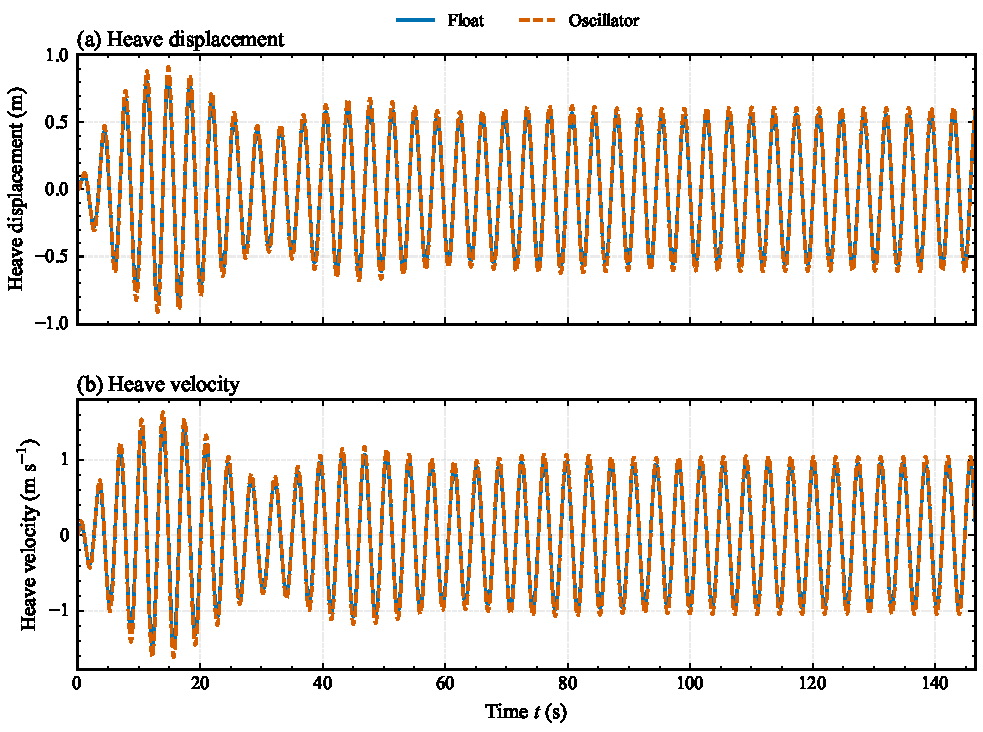
\includegraphics[width=0.95\textwidth]{q3_heave_response.pdf}
  \caption{情形 3 下浮子与振子的垂荡位移和速度响应}
  \label{fig:q3-heave}
\end{figure}

\begin{figure}[H]
  \centering
  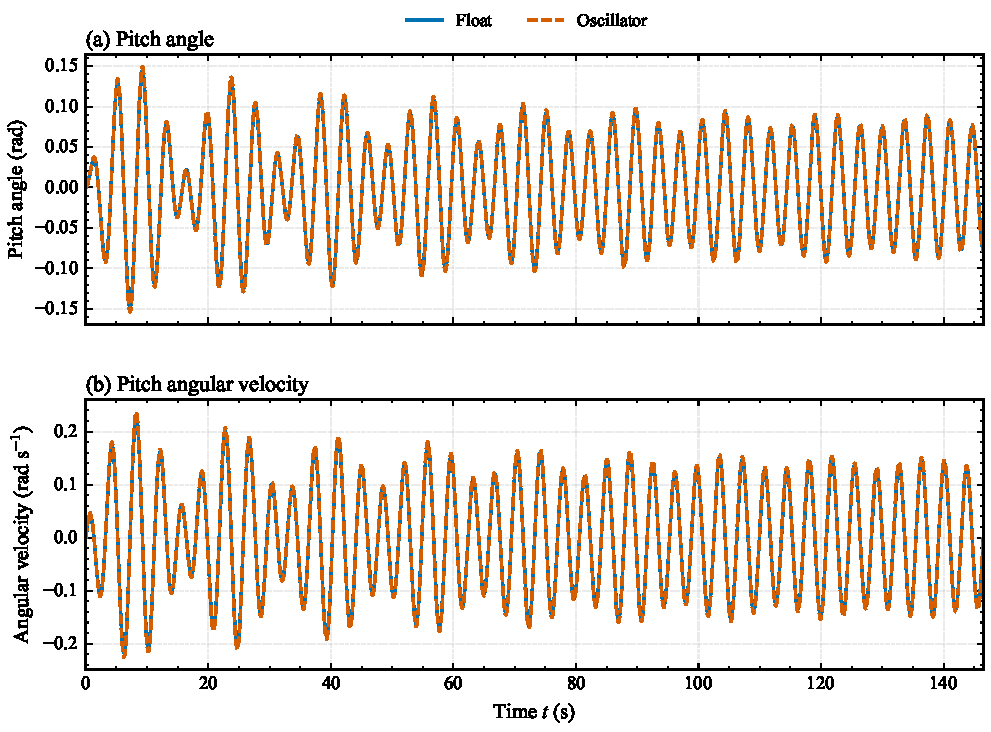
\includegraphics[width=0.95\textwidth]{q3_pitch_response.pdf}
  \caption{情形 3 下浮子与振子的纵摇角和角速度响应}
  \label{fig:q3-pitch}
\end{figure}

题目指定的 $10$、$20$、$40$、$60$ 和 $100\ \mathrm{s}$ 时刻的垂荡结果见表 \ref{tab:q3-heave-results}，纵摇结果见表 \ref{tab:q3-pitch-results}。

\begin{table}[H]
  \centering
  \small
  \caption{问题三指定时刻的垂荡响应}
  \label{tab:q3-heave-results}
  \begin{tabular}{ccccc}
    \toprule
    时间/s & 浮子位移/m & 浮子速度/(m/s) & 振子位移/m & 振子速度/(m/s) \\
    \midrule
    10  & -0.5283 &  0.9699 & -0.5987 &  1.0382 \\
    20  & -0.7048 & -0.2693 & -0.7723 & -0.3190 \\
    40  &  0.3694 &  0.7576 &  0.3927 &  0.8450 \\
    60  & -0.3207 & -0.7218 & -0.3414 & -0.7993 \\
    100 & -0.0502 & -0.9467 & -0.0426 & -1.0365 \\
    \bottomrule
  \end{tabular}
\end{table}

\begin{table}[H]
  \centering
  \small
  \caption{问题三指定时刻的纵摇响应}
  \label{tab:q3-pitch-results}
  \begin{tabular}{ccccc}
    \toprule
    时间/s & 浮子角/rad & 浮子角速度/(rad/s) & 振子角/rad & 振子角速度/(rad/s) \\
    \midrule
    10  &  0.0550 & -0.1978 &  0.0572 & -0.2049 \\
    20  &  0.0863 & -0.0456 &  0.0894 & -0.0474 \\
    40  & -0.1082 & -0.0764 & -0.1121 & -0.0791 \\
    60  &  0.0475 &  0.1198 &  0.0491 &  0.1242 \\
    100 &  0.0381 &  0.1186 &  0.0394 &  0.1227 \\
    \bottomrule
  \end{tabular}
\end{table}

全过程浮子和振子的最大垂荡位移绝对值分别约为 $0.831\ \mathrm{m}$ 和 $0.916\ \mathrm{m}$，最大纵摇角绝对值分别约为 $0.148\ \mathrm{rad}$ 和 $0.154\ \mathrm{rad}$。最大纵摇角约为 $8.81^\circ$，未超过本文设定的 $0.2\ \mathrm{rad}$ 小角度预警线。

\subsection{PTO 输出与能量特征}

直线与旋转 PTO 的瞬时输出功率分别为
\begin{equation}
  P_z=10000(\dot x_o-\dot x_f)^2\geq0,
  \qquad
  P_\theta=1000(\dot\theta_o-\dot\theta_f)^2\geq0.
  \label{eq:q3-pto-power}
\end{equation}
至精确第 $40$ 周期终点，直线 PTO 和旋转 PTO 的累计输出能量分别约为 $6.94\ \mathrm{kJ}$ 和 $1.93\ \mathrm{J}$，瞬时功率最大值分别约为 $245.43\ \mathrm{W}$ 和 $0.070\ \mathrm{W}$。旋转 PTO 输出比直线 PTO 小三个数量级以上，说明在题给阻尼参数下，装置能量输出主要来自垂荡方向的直线 PTO。

\begin{figure}[H]
  \centering
  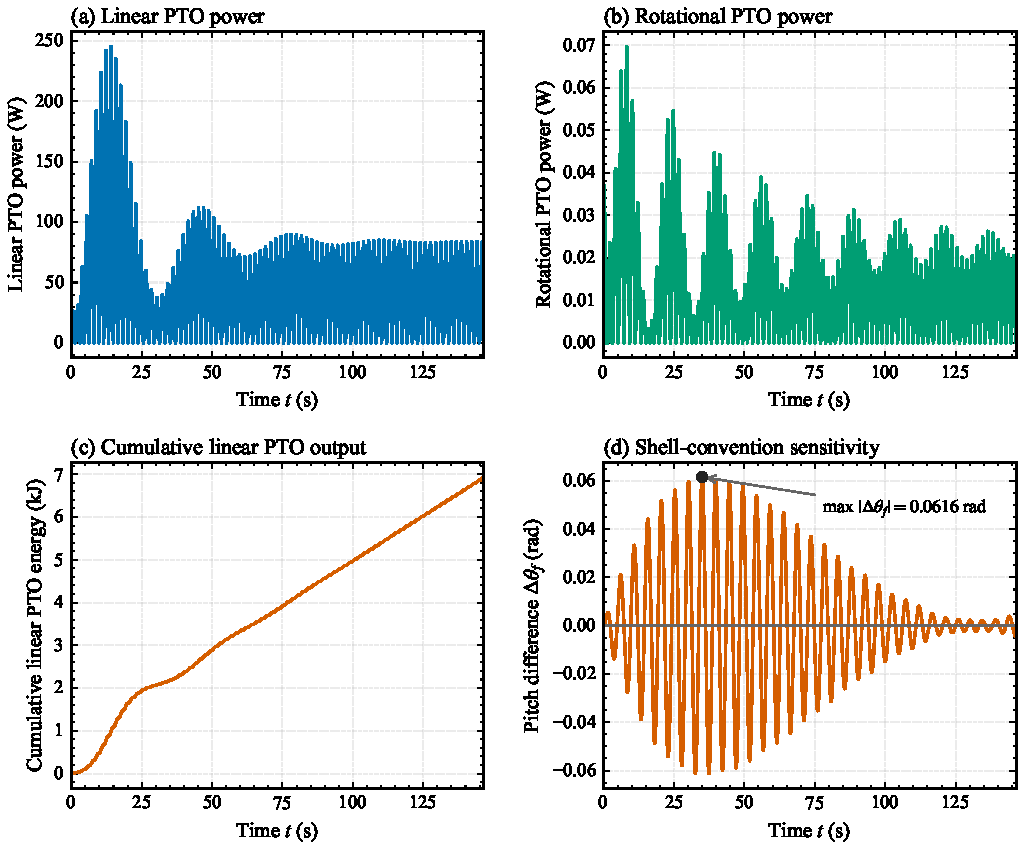
\includegraphics[width=0.95\textwidth]{q3_pto_and_sensitivity.pdf}
  \caption{两类 PTO 输出与浮子壳体口径敏感性}
  \label{fig:q3-pto-sensitivity}
\end{figure}

\subsection{数值验证与模型敏感性}

问题三的结果采用收紧步长的积分、常系数系统的矩阵指数解和能量恒等式交叉验证。三条独立路径在机器精度范围内一致；将波浪输入功、机械能变化、垂荡与纵摇兴波耗散以及两类 PTO 输出纳入能量恒等式，终点相对残差低于 $10^{-12}$。

全过程弹簧长度约保持在 $0.115$--$0.289\ \mathrm{m}$，始终为正；最大纵摇角也低于小角度预警线，因此结构几何和一阶线性化在主响应范围内自洽。

由于题面未明确薄壳是否包含顶部圆盖，另以“不计顶部圆盖”的侧壳口径进行敏感性计算。图 \ref{fig:q3-pto-sensitivity}(d) 中 $\Delta\theta_f$ 表示“替代口径减主口径”。两种口径下四个垂荡状态完全不变，纵摇绝对峰值变化约 $1\%$--$2\%$；但由于低阻尼模态存在瞬态相位累积，两种口径的纵摇角最大逐时差约为 $0.06\ \mathrm{rad}$。因此纵摇峰值规模对壳体口径较稳健，而低阻尼纵摇瞬态的相位对转动惯量口径较敏感。主结果始终采用计入顶部圆盖的封闭薄壳口径，替代口径不混入正式结果表。

\section{问题四直线与旋转 PTO 阻尼联合优化}

\subsection{情形 4 参数与频域目标}

问题四采用附件 3 的情形 4，水动力参数为
\begin{equation}
  \omega=1.9806\ \mathrm{s^{-1}},\quad
  m_a=1091.099\ \mathrm{kg},\quad
  J_a=7142.493\ \mathrm{kg\,m^2},
  \label{eq:q4-hydrodynamic-1}
\end{equation}
\begin{equation}
  b_z=528.5018\ \mathrm{N\,s/m},\quad
  b_\theta=1655.909\ \mathrm{N\,m\,s},\quad
  F=1760\ \mathrm{N},\quad L=2140\ \mathrm{N\,m}.
  \label{eq:q4-hydrodynamic-2}
\end{equation}
沿用问题三的封闭薄壳口径和四自由度一阶模型，仅将水动力参数替换为情形 4。记直线和旋转 PTO 阻尼系数为 $c_z,c_\theta$，二者均满足
\begin{equation}
  0\leq c_z\leq100000,\qquad 0\leq c_\theta\leq100000.
  \label{eq:q4-bounds}
\end{equation}

对 $j\in\{z,\theta\}$，令 $\boldsymbol r=[1,-1]^{\mathsf T}$，设周期稳态位移为 $\boldsymbol q_j(t)=\Re\{\boldsymbol X_j\mathrm e^{\mathrm i\omega t}\}$，则复振幅满足
\begin{equation}
  \left[\boldsymbol K_j-\omega^2\boldsymbol M_j+
  \mathrm i\omega\left(\boldsymbol C_{j,0}+c_j\boldsymbol r\boldsymbol r^{\mathsf T}\right)\right]
  \boldsymbol X_j=\boldsymbol F_j,
  \label{eq:q4-frequency-system}
\end{equation}
其中 $\boldsymbol C_{j,0}$ 仅包含浮子的兴波阻尼。两类 PTO 的周期平均功率为
\begin{equation}
  \overline P_j(c_j)=\frac12c_j\omega^2
  \left|\boldsymbol r^{\mathsf T}\boldsymbol X_j\right|^2,
  \qquad j\in\{z,\theta\}.
  \label{eq:q4-component-power}
\end{equation}
一阶模型中垂荡与纵摇两个子系统分离，因此联合目标可严格写成
\begin{equation}
  \boxed{\overline P(c_z,c_\theta)=\overline P_z(c_z)+\overline P_\theta(c_\theta)}.
  \label{eq:q4-total-power}
\end{equation}
这一分解是由块对角动力学结构导出的精确结果，而非忽略两类 PTO 之间影响的近似。

\subsection{解析最优条件}

对任一子系统，定义
\begin{equation}
  \boldsymbol Z_0=\boldsymbol K-\omega^2\boldsymbol M+
  \mathrm i\omega\boldsymbol C_0,
  \quad
  \alpha=\boldsymbol r^{\mathsf T}\boldsymbol Z_0^{-1}\boldsymbol F,
  \quad
  s=\boldsymbol r^{\mathsf T}\boldsymbol Z_0^{-1}\boldsymbol r.
  \label{eq:q4-rank-one-definitions}
\end{equation}
应用 Sherman--Morrison 秩一更新公式\cite{sherman1950}，得到相对位移复振幅和平均功率
\begin{equation}
  \boldsymbol r^{\mathsf T}\boldsymbol X(c)
  =\frac{\alpha}{1+\mathrm i\omega cs},
  \qquad
  \overline P(c)=
  \frac{\tfrac12c\omega^2|\alpha|^2}{|1+\mathrm i\omega cs|^2}.
  \label{eq:q4-rank-one-power}
\end{equation}
对 $c$ 求导后，导数符号仅取决于 $1-\omega^2|s|^2c^2$，故无约束正最优点为
\begin{equation}
  \boxed{c_0^*=\frac{1}{\omega|s|}}.
  \label{eq:q4-analytic-optimum}
\end{equation}
将两个无约束最优点分别投影到式 \eqref{eq:q4-bounds} 的可行区间，即得联合问题的约束全局最优解。两个子系统在完整可行区间的功率曲线见图 \ref{fig:q4-curves}。

\begin{figure}[H]
  \centering
  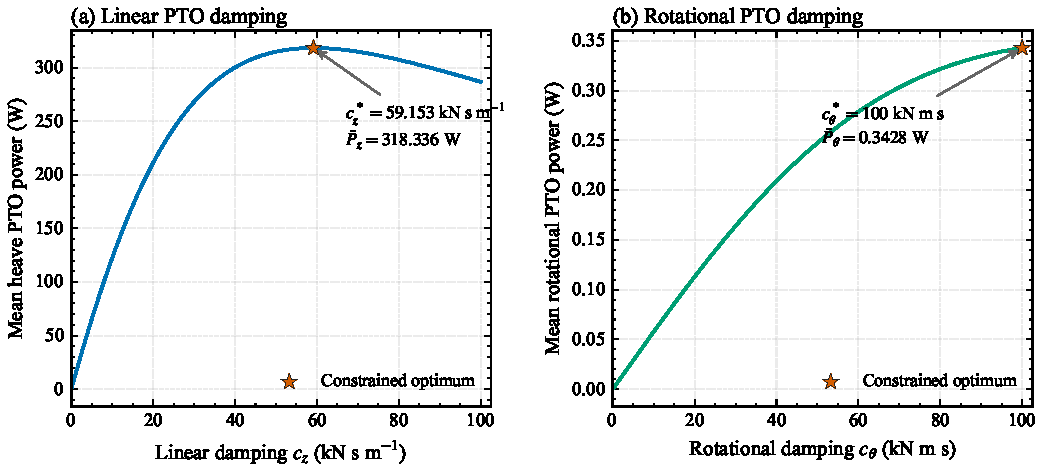
\includegraphics[width=0.94\textwidth]{q4_optimization_curves.pdf}
  \caption{直线与旋转 PTO 常量阻尼的周期稳态平均功率曲线}
  \label{fig:q4-curves}
\end{figure}

直线阻尼的无约束最优点为 $5.9153\times10^4\ \mathrm{N\,s/m}$，位于区间内部；旋转阻尼的无约束最优点约为 $1.2011\times10^5\ \mathrm{N\,m\,s}$，超过题设上限。因此旋转阻尼在可行区间内随系数增大而增功，$c_\theta=1.0000\times10^5$ 为活跃上边界。

\subsection{最优结果与全局性验证}

问题四的最优阻尼与平均功率见表 \ref{tab:q4-optima}。

\begin{table}[H]
  \centering
  \caption{问题四的最优阻尼与平均功率}
  \label{tab:q4-optima}
  \begin{tabular}{lc}
    \toprule
    指标 & 最优值 \\
    \midrule
    直线阻尼系数 $c_z^*$ & $5.9153\times10^4\ \mathrm{N\,s/m}$ \\
    旋转阻尼系数 $c_\theta^*$ & $1.0000\times10^5\ \mathrm{N\,m\,s}$ \\
    直线 PTO 平均功率 & $318.336\ \mathrm{W}$ \\
    旋转 PTO 平均功率 & $0.343\ \mathrm{W}$ \\
    最大总平均功率 & $318.679\ \mathrm{W}$ \\
    单周期总输出能量 & $1010.97\ \mathrm{J}$ \\
    \bottomrule
  \end{tabular}
\end{table}

旋转 PTO 仅占总平均功率的 $0.108\%$，表明情形 4 中装置输出主要由垂荡相对运动贡献。为排除解析分解和单峰判断带来的路径依赖，本文对两个阻尼区间分别进行全域扫描和有界连续优化，并在完整二维参数域内独立执行差分进化搜索。二维数值搜索得到的阻尼系数与总功率均与解析约束最优值一致。图 \ref{fig:q4-surface} 以对数色标给出参数域内相对最优点的功率损失 $\overline P_{\max}-\overline P$，图中色值并非总功率本身。

\begin{figure}[H]
  \centering
  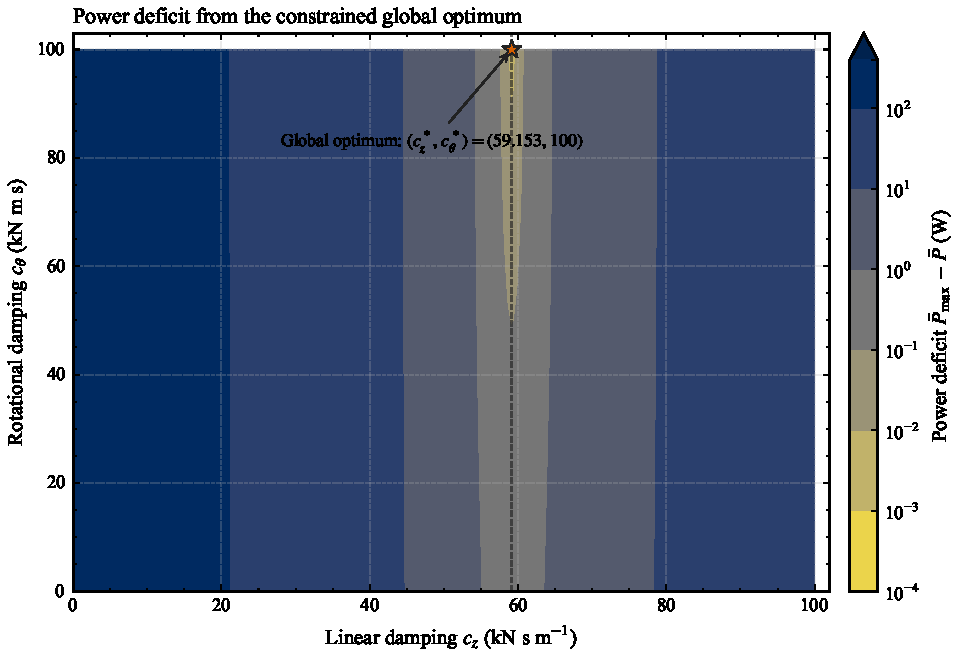
\includegraphics[width=0.92\textwidth]{q4_total_power_surface.pdf}
  \caption{联合阻尼参数域内相对约束全局最优点的平均功率损失}
  \label{fig:q4-surface}
\end{figure}

另对两个最优阻尼系数分别作 $1$、$10$、$100$ 和 $1000$ 的可行邻域扰动，所有扰动点的总功率均低于表 \ref{tab:q4-optima} 中的结果，从局部方向进一步验证了内部最优点和活跃边界的正确性。

\subsection{最优周期响应与能量闭合}

将频域最优解转换为周期初态，再以 DOP853 方法进行时域积分。最优周期内的相对运动和两类 PTO 瞬时功率如图 \ref{fig:q4-period} 所示。

\begin{figure}[H]
  \centering
  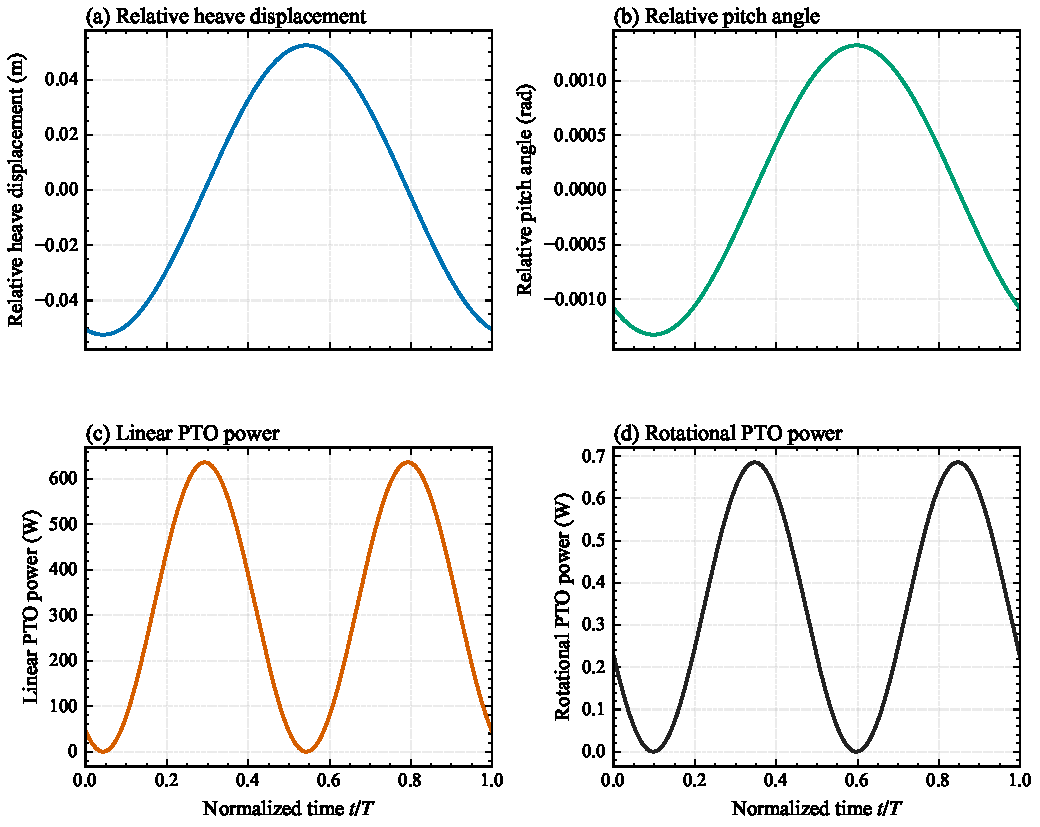
\includegraphics[width=0.94\textwidth]{q4_optimal_period_response.pdf}
  \caption{最优阻尼参数下一个稳定波浪周期的相对运动与 PTO 瞬时功率}
  \label{fig:q4-period}
\end{figure}

垂荡相对位移和速度振幅分别约为 $0.0524\ \mathrm{m}$ 和 $0.1037\ \mathrm{m/s}$，纵摇相对角和角速度振幅分别约为 $1.32\times10^{-3}\ \mathrm{rad}$ 和 $2.62\times10^{-3}\ \mathrm{rad/s}$。直线和旋转 PTO 的瞬时最大功率分别约为 $636.67\ \mathrm{W}$ 和 $0.686\ \mathrm{W}$。

周期平均能量分配如表 \ref{tab:q4-energy} 所示。

\begin{table}[H]
  \centering
  \caption{最优周期的平均功率分配}
  \label{tab:q4-energy}
  \begin{tabular}{lc}
    \toprule
    平均功率项 & 数值/W \\
    \midrule
    波浪输入 & 911.992 \\
    垂荡兴波耗散 & 583.575 \\
    直线 PTO 输出 & 318.336 \\
    纵摇兴波耗散 & 9.737 \\
    旋转 PTO 输出 & 0.343 \\
    \bottomrule
  \end{tabular}
\end{table}

周期首尾状态闭合，时域总平均功率、频域结果与平均能量平衡在机器精度范围内一致。弹簧长度约保持在 $0.150$--$0.254\ \mathrm{m}$，圆柱段吃水约保持在 $1.250$--$2.750\ \mathrm{m}$，最大绝对纵摇角约为 $0.0558\ \mathrm{rad}$，均满足本文的物理适用性条件。

\section{模型评价与推广}

\subsection{模型优点}

\begin{enumerate}[leftmargin=3.2em]
  \item \textbf{物理口径统一。} 四问均以静水平衡位置为基准，弹簧力和 PTO 阻尼力始终作为系统内力成对出现；功率统一按阻尼耗散定义，保证动力学方程与能量计算具有一致的符号约定。
  \item \textbf{优化目标可比。} 问题二和问题四均采用单个周期稳态平均功率，排除了初始自由振动对阻尼参数优劣的干扰；常量阻尼使用频域解析解，幂律阻尼使用周期射击，使线性与非线性工况在同一评价尺度下比较。
  \item \textbf{验证链条完整。} 关键结果同时经过步长与容差收敛、频域或矩阵指数独立解、能量闭合、全域扫描及最优点邻域扰动检验。模型不仅给出数值，还说明了最优解的唯一性、活跃边界及物理适用范围。
\end{enumerate}

\subsection{模型局限}

\begin{enumerate}[leftmargin=3.2em]
  \item 水动力系数按题设视为定常线性参数，未考虑大幅运动下附加质量、兴波阻尼随频率和振幅变化，也未计入黏性阻力、系泊系统及 PTO 机械效率。
  \item 垂荡--纵摇模型采用微幅波和小角度一阶线性化。问题三最大纵摇角约为 $8.81^\circ$，仍在本文预警线内，但已提示在更强海况下应改用非线性几何和时变水动力模型。
  \item 题面未完全规定浮子内部质量分布。本文以均匀封闭薄壳为主口径，并通过替代壳体口径给出敏感性分析；因此纵摇瞬态相位应结合实际结构惯量进一步校准。
\end{enumerate}

\subsection{模型推广}

本文框架可直接推广到多频不规则波：将规则波激励替换为波谱离散叠加，在足够长的统计窗口内计算平均功率与载荷极值；也可把常量阻尼扩展为分段、饱和或可控阻尼，并增加位移、速度和峰值载荷约束，形成面向真实 PTO 控制器的多目标优化。若获得试验或实海数据，还可通过参数辨识更新附加质量、兴波阻尼和转动惯量，并沿用本文的能量闭合与独立求解路径进行模型校验。

\section{结论}

本文建立了波浪周期激励下浮子--振子系统的二自由度垂荡耦合模型，完成了常量与幂律阻尼下的时域响应计算，并通过收敛、能量和几何范围检验验证了模型可靠性。在此基础上，将平均输出功率统一定义为周期稳态口径，分别得到常量阻尼的唯一内部最优点和幂律阻尼的边界最优点。幂律阻尼的最大平均功率较常量阻尼提高约 $0.288\%$，但比例系数已取到允许上界，说明参数域的边界对最优解具有决定作用。

对垂荡--纵摇联合运动，本文通过壳体几何和平行轴定理补全转动惯量，建立了四自由度线性动力学模型。题给阻尼参数下，装置能量输出主要来自垂荡方向的直线 PTO，旋转 PTO 输出较小。数值积分、矩阵指数解与能量闭合结果一致，并且主响应满足小角度与结构几何范围。壳体敏感性分析同时表明，峰值规模较稳健，但低阻尼纵摇瞬态的相位结论应对转动惯量口径保持谨慎。

在垂荡与纵摇联合优化中，本文利用一阶模型的块对角结构将二维总功率目标严格分解，并以秩一更新得到解析最优条件。最优直线阻尼为 $5.9153\times10^4\ \mathrm{N\,s/m}$，最优旋转阻尼取上边界 $1.0000\times10^5\ \mathrm{N\,m\,s}$，最大总平均功率为 $318.679\ \mathrm{W}$。解析推导、穷举扫描、二维差分进化与周期时域能量闭合相互一致，使最终结果同时具备全局最优性、数值可复现性和物理自洽性。

\begin{thebibliography}{99}
\small
\setlength{\itemsep}{0.35em}
  \bibitem{falnes2002}
  Falnes J. \emph{Ocean Waves and Oscillating Systems: Linear Interactions Including Wave-Energy Extraction}[M]. Cambridge: Cambridge University Press, 2002.

  \bibitem{cummins1962}
  Cummins W E. The impulse response function and ship motions[J]. \emph{Schiffstechnik}, 1962, 9(47): 101--109.

  \bibitem{hairer1993}
  Hairer E, N{\o}rsett S P, Wanner G. \emph{Solving Ordinary Differential Equations I: Nonstiff Problems}[M]. 2nd ed. Berlin: Springer, 1993.

  \bibitem{sherman1950}
  Sherman J, Morrison W J. Adjustment of an inverse matrix corresponding to a change in one element of a given matrix[J]. \emph{The Annals of Mathematical Statistics}, 1950, 21(1): 124--127.
\end{thebibliography}

\clearpage
\begin{appendices}

\section{支撑材料与结果文件说明}

问题一两种阻尼工况的 $898$ 个完整输出时刻已分别写入下列官方格式结果表：
\begin{itemize}[leftmargin=3.2em]
  \item \path{result1-1.xlsx}：常量阻尼完整结果；
  \item \path{result1-2.xlsx}：幂律阻尼完整结果。
\end{itemize}
正文表 \ref{tab:linear-results} 和表 \ref{tab:power-results} 均直接取自上述文件。问题二的最终参数、功率、周期指标和验收状态汇总于支撑材 \path{q2_final_summary.json}。问题三的 $733\times9$ 正式结果位于 \path{result3.xlsx}，正文表 \ref{tab:q3-heave-results} 和表 \ref{tab:q3-pitch-results} 的指定时刻数值均取自该工作簿；问题三最终汇总为 \path{q3_final_summary.json}。问题四无额外官方结果表，其解析最优解、独立搜索结果、周期响应及验收状态汇总于 \path{q4_final_summary.json}。

代码附录按“每问主求解入口”给出，完整工程还包含以下支撑模块：
\begin{itemize}[leftmargin=3.2em]
  \item \path{code/common/q1_dynamics.py}：问题一统一动力学与能量计算；
  \item \path{code/common/q2_power.py}：问题二频域功率和周期射击计算；
  \item \path{code/common/q3_dynamics.py}：问题三和问题四的四自由度动力学；
  \item \path{code/common/q4_power.py}：问题四频域功率与解析最优条件；
  \item \path{code/q1}–\path{code/q4} 中的 \path{verify_*.py} 和绘图脚本：回归测试、交付核验与正式图生成。
\end{itemize}

\section{问题一核心求解代码}
\lstinputlisting[
  language=Python,
  caption={问题一两类阻尼工况的时域求解与结果导出}
]{../code/q1/solve_q1.py}

\section{问题二常量阻尼优化代码}
\lstinputlisting[
  language=Python,
  caption={问题二常量阻尼的全区间扫描与频域优化}
]{../code/q2/optimize_q2_constant.py}

\section{问题二幂律阻尼优化代码}
\lstinputlisting[
  language=Python,
  caption={问题二幂律阻尼的边界精修与周期独立验证}
]{../code/q2/validate_q2_nonlinear_final.py}

\section{问题三核心求解与验证代码}
\lstinputlisting[
  language=Python,
  caption={问题三四自由度响应、能量闭合与壳体敏感性验证}
]{../code/q3/validate_q3_full.py}

\section{问题四联合阻尼优化代码}
\lstinputlisting[
  language=Python,
  caption={问题四解析优化、二维独立搜索与周期时域复核}
]{../code/q4/optimize_q4.py}

\end{appendices}

\end{document}
